 \documentclass{report}
 
\usepackage[utf8]{inputenc} 
\usepackage[T1]{fontenc}      
\usepackage[top=2.0cm, bottom=3cm, left=3.0cm, right=3.0cm]{geometry}
\usepackage{graphicx}
\usepackage{wrapfig}
\usepackage{amsmath,esint }
\usepackage{amssymb}
\graphicspath{{figures/}{../figures}}

\newcommand*\dif{\mathop{}\!\mathrm{d}}
\newcommand*\diver{\mathop{}\!\mathrm{div}}
\newcommand*\grad{\mathop{}\!\mathrm{grad}}

\begin{document}

\section*{Étude d'une corde}

On considère une corde suspendue entre deux points fixes de même hauteur $y=0$, situés à $x=-D/2$ et $x=+D/2$. La corde a une masse volumique $\mu$.

\subsubsection{Cas statique}

La corde est supposée dans un premier temps statique.

\begin{figure}[h!]
\centering
		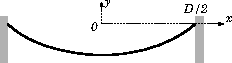
\includegraphics[scale=1.5]{onde1.pdf}
\end{figure}

\begin{itemize}

	\item[$\star$] En appliquant le principe fondamental de la statique sur un élément de corde, déterminer une équation différentielle en $y(x)$, correspondant à la hauteur $y$ de la corde à l'abscisse $x$. On fera apparaître une longueur caractéristique $l_c$, dont on précisera l'expression.
	
	\item[$\star$] Résoudre cette équation différentielle (on pourra résoudre l'équation en utilisant le changement de variable $p(x)=\dif y/\dif x$). Trouver la solution à l'aide des conditions aux limites. 
	
	\item[$\star$] Déterminer la tension $T(x)$ le long de la corde. A quelle endroit est-elle maximale ? Minimale ? Commenter. 
	
	\item[$\star$] Exprimer la longueur $L$ et la \textit{flèche} $h$ (la hauteur entre le point le plus haut et le plus bas) de la chaîne en fonction du paramètre $l_c$. Comment connaître alors la tension dans une chaîne suspendue simplement à partir d'une photographie de celle-ci et de sa masse linéique ?
	
\end{itemize}

\subsubsection*{Cas dynamique}

On considère maintenant que la corde est fortement tendue mais qu'elle n'est plus statique. On cherche à comprendre sa dynamique. On négligera les frottements.

\begin{itemize}

	\item[$\diamond$] Que se passe t-il lorsque la corde devient extrêmement tendue ? Que peut-on négliger par rapport au cas statique ?

	\item[$\diamond$] Déterminer l'équation régissant $y(x,t)$ le long de la corde. Comment s'appelle cette équation ? Quelles sont ses solutions ? Commenter.
	
	\item[$\diamond$] Sachant que la corde est ancrée en $x=0$ et $x=L$, donner l'expression générale de $y(x,t)$ dans le cas de solutions stationnaires. 
	
	\item[$\diamond$] On excite la corde avec une excitation dessinée ci-dessous. Donner l'expression de $y(x,t)$ dans ce cas-là.
	
	\begin{figure}[h!]
	\centering
		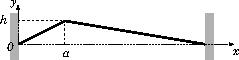
\includegraphics[scale=1.5]{onde2.pdf}
	\end{figure}

	\item[$\diamond$] Si la corde décrite dans l'exercice est celle d'un instrument de musique (violon, guitare, piano...), comment expliquer la différence de timbre entre ces instruments pour une note donnée ?
	
\end{itemize}

\newpage

\section*{Corde pendue verticalement}

On considère une corde attachée au plafond à un point fixe et laissée verticalement à elle-même dans le vide. On prendra pour origine $z=0$ le bout de la corde. Elle n'est soumise qu'à la gravité. On notera $\Psi(z,t)$ l'écart de la corde à la verticale à la hauteur $z$ à l'instant $t$, que l'on supposera très petit par rapport à la longueur $L$ de la corde.

\begin{figure}[h!]
\centering
	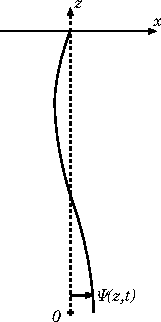
\includegraphics[scale=1.5]{onde4.pdf}
\end{figure}


\begin{itemize}

	\item[$\ast$] En appliquant le principe fondamental de la dynamique, trouver une équation différentielle en  $\Psi(z,t)$.

\end{itemize}

On cherche des solutions sous la forme $\Psi(z,t)=\alpha(z)\cos(\omega t)+\beta(z)\sin(\omega t)$. 

\begin{itemize}
	
		\item[$\ast$] Comment s'appellent ce type de solutions ? Déterminer l'équation différentielle vérifiée par $\alpha$ et $\beta$.
		
		\item[$\ast$] En posant $Z=\frac{z\omega^2}{g}$, trouver un nouveau système d'équation différentielle en $A(Z)=\alpha(z)/\alpha(0)$. 
		
		\item[$\ast$] On cherche la solution sous la forme d'une série entière $A(Z)=\sum_k A_k Z^K$. Déterminer les coefficients $K$. 
		
		\item[$\ast$] Comment pourrait-on trouver une relation de dispersion $\omega(k)$ ?
		
\end{itemize}

\newpage

\section*{Propagation sur une ligne électrique}

On considère une ligne électrique composée d'une suite de cellules identiques, constituées d'une inductance $L$ et d'une capacité $C$ comme indiqué sur le schéma ci-dessous. Dans la cellule $n$, on note $V_n$ la tension au bornes de la capacité et $I_n$ le courant traversant  l'inductance.

\begin{figure}[h!]
\centering
	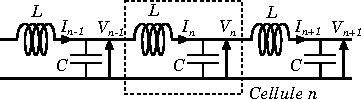
\includegraphics[scale=1.5]{onde3.pdf}
\end{figure}

\begin{itemize}

	\item[$\spadesuit$] En établissant des relations entre les courants et les tensions des cellules $n-1$, $n$ et $n+1$, montrer que la tension $V_n$ vérifie la relation suivante :
	\begin{equation}
		\frac{\dif^2 V_n}{\dif t^2} =\omega_0^2(V_{n+1}+V_{n-1}-2V_n)
		\label{eq:prop}
	\end{equation}
	On précisera l'expression de $\omega_0$.
	
	 \item[$\spadesuit$] Calculer la quantité $\frac{\dif}{\dif t}\left( \frac{1}{2}CV_n^2 + LI_n^2 \right) $. Interpréter physiquement l'ensemble des termes.

\end{itemize}

On cherche une solution sinusoïdale pour $V_n(t)$ de l'équation \ref{eq:prop} (on prendra la notation complexe $V_n(t)=A_n\exp(j\omega t)$) de sorte à ce que l'effet après le passage dans une cellule soit un déphasage $\alpha$ fixé : $V_{n+1}=V_n\exp(-j\alpha)$, avec $\alpha>0$.

\begin{itemize}

	\item[$\spadesuit$] Quelle est la signification de la grandeur $\alpha$ en terme de propagation ? Exprimer $A_n$ en fonction de $A_0$, $n$ et $\alpha$. En déduire une relation de "dispersion" entre $\omega$ et $\alpha$.

	\item[$\spadesuit$] Montrer que ces solutions n'existent que si $\omega$ est inférieur à une certaine fréquence $\omega_c$, que l'on exprimera. Si cette condition est vérifiée, pourquoi peut-on parler de propagation de la phase ? Préciser la vitesse de propagation $v_\varphi$ correspondante.
	
	\item[$\spadesuit$] On suppose maintenant que $\omega\ll\omega_c$. En explicitant $\alpha$ en fonction de $\omega$, exprimer $v_\varphi$. Que constate t-on ? En déduire l'effet d'une cellule sur un signal électrique, composé de fréquence suffisamment basses, se traduit par un retard temporel $\tau$ que l'on exprimera en fonction de $\omega_0$. Application numérique : $C=10$nF et $L=25\mu$H, calculer $\omega_0$ et $\tau$. Combien de cellules doit-on mettre pour obtenir un retard de $0.1$ms ?

	\item[$\spadesuit$] On se place dans le cas où $\omega<\omega_c$ et $\alpha>0$. Rappeler la définition et l'interprétation de la vitesse de groupe. En donner l'expression en fonction de $\omega_0$ et $\alpha$ et donner son allure de son graphe en fonction de $\alpha$. Que se passe t-il pour $\alpha=\pi$ ?
	
	\item[$\spadesuit$] En notation complexe, l'intensité $I_n$ est de la forme $I_n(t)=B_n\exp(j\omega t)$. Exprimer $B_n$ en fonction de $A_n$, $L$, $\omega_0$ et $\alpha$. Calculer la moyenne temporelle de l'énergie de la cellule $n$ $E=\left\langle \frac{1}{2}CV_n^2+\frac{1}{2}LI_n^2\right\rangle$, ainsi que celle de la puissance $P$ reçue par la cellule $n-1$. En déduire le rapport $P/E$. Commenter.  	

\end{itemize}

\subsubsection*{Question supplémentaire}

On suppose que l'inductance $L$ et la capacité $C$ sont remplacées respectivement par une inductance linéique $\Lambda$ et une capacité linéique $\Gamma$. 

\begin{itemize}

	\item[$\heartsuit$] En substituant judicieusement l'indice $n$ par la dimension spatiale $x$ le long du câble coaxial, montrer que l'équation \ref{eq:prop} devient une équation d'Alembert.
	
	\item[$\heartsuit$] Dans ce cas-là, par quelle quantité substituer $\alpha$ ? Sur quel type de solutions sur $V$ retombe t-on ? Que devient l'équation de dispersion ? Justifier. 

\end{itemize}

\end{document}
